% Propósito: enseñar a leer el campo audible como una región dependiente de
% frecuencia, procedimiento y población, y no como dos límites universales.
% Origen: descripción cualitativa de la sección
% \ref{sec:u7-umbral-absoluto}. Las curvas son esquemáticas, no datos
% experimentales ni límites normativos.
% Descripción accesible: un eje horizontal cualitativo representa la frecuencia
% en hertz y uno vertical el nivel de presión sonora en dB SPL. Una frontera
% inferior ondulada representa el umbral y posee una zona de menor nivel en
% frecuencias medias. Una frontera superior representa niveles elevados que no
% deben explorarse en actividades. El área entre ambas se rotula campo audible.
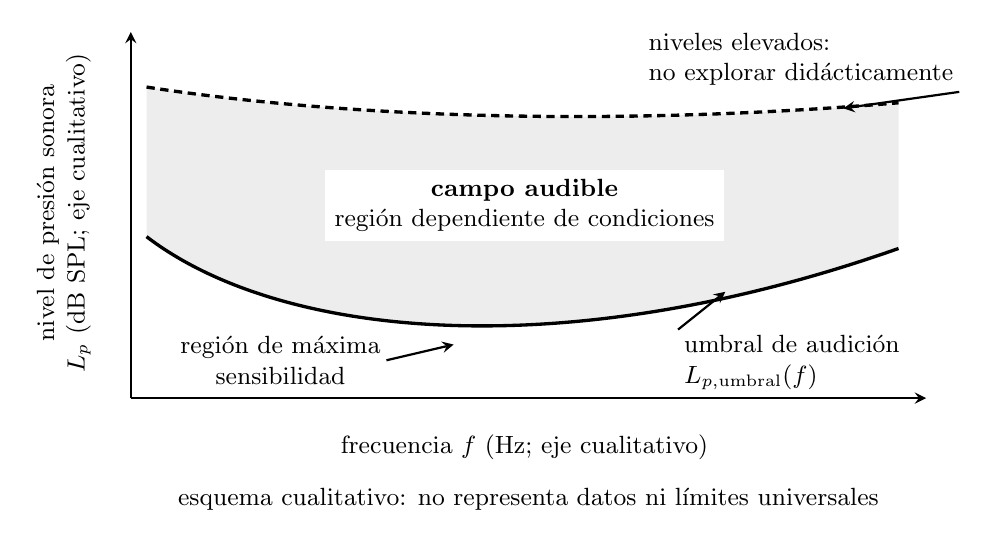
\begin{tikzpicture}[font=\small,>=stealth,x=1cm,y=1cm]
    \draw[->,thick] (1.10,0.80) -- (11.20,0.80);
    \draw[->,thick] (1.10,0.80) -- (1.10,5.45);
    \node at (6.10,0.18)
        {frecuencia \(f\) (Hz; eje cualitativo)};
    \node[rotate=90,align=center] at (0.25,3.15)
        {nivel de presión sonora\\\(L_p\) (dB SPL; eje cualitativo)};

    \path[fill=black!7]
        (1.30,2.85)
        .. controls (3.00,1.55) and (6.60,1.20) .. (10.85,2.70)
        -- (10.85,4.55)
        .. controls (7.30,4.25) and (3.90,4.35) .. (1.30,4.75)
        -- cycle;

    \draw[very thick]
        (1.30,2.85)
        .. controls (3.00,1.55) and (6.60,1.20) .. (10.85,2.70);
    \draw[very thick,densely dashed]
        (1.30,4.75)
        .. controls (3.90,4.35) and (7.30,4.25) .. (10.85,4.55);

    \node[fill=white,align=center] at (6.10,3.25)
        {\textbf{campo audible}\\
         región dependiente de condiciones};
    \node[anchor=west,align=left,fill=white,inner sep=2pt]
        (threshold-label) at (8.05,1.25)
        {umbral de audición\\
         \(L_{p,\mathrm{umbral}}(f)\)};
    \draw[->,thick]
        (threshold-label.north west) -- (8.65,2.15);

    \node[anchor=west,align=left,fill=white,inner sep=2pt]
        (upper-label) at (7.60,5.10)
        {niveles elevados:\\
         no explorar didácticamente};
    \draw[->,thick]
        (upper-label.south east) -- (10.15,4.48);

    \node[align=center,fill=white,inner sep=2pt]
        (sensitivity-label) at (3.00,1.28)
        {región de máxima\\sensibilidad};
    \draw[->,thick]
        (sensitivity-label.east) -- (5.20,1.48);

    \node[align=center] at (6.15,-0.48)
        {esquema cualitativo: no representa datos ni límites universales};
\end{tikzpicture}
